\chapter{General Context and Introduction}

\section{Introduction}
MapIT is a full-stack application built to support the documentation of IT infrastructure, the management of incidents and assets, the mapping of relationships, and the reuse of technical knowledge. Rather than behaving like a generic document repository, the platform follows the daily logic of an IT support team: identify the asset, understand its dependencies, record the incident, preserve the resolution, and make that knowledge searchable for later reuse. This chapter situates the project in its real environment, states the problem it addresses, and explains why the topic matters both academically and professionally.
\section{Host Organization: SNTF}
\subsection{Short presentation}
SNTF stands for \emph{Société nationale des transports ferroviaires}, the Algerian state-owned company providing passenger and freight services using its extensive rail network. As per the company's official presentations, the SNTF was created in 1976, and reorganized in 1990 to become an EPIC entity.
\subsection{Visual identity}
Figure~\ref{fig:sntf-logo} presents the official SNTF logo used as a visual reference for the host organization.

\begin{figure}[H]
	\centering
	
\includegraphics[width=0.62\textwidth]{figures/sntf.png}
	\caption{Official logo of SNTF}
	\label{fig:sntf-logo}
\end{figure}

\subsection{DSI organigramme}
The DSI organigramme shows how the Information Systems Department is organized around several complementary missions: project management, network administration, systems development, web activities, database administration, security-oriented messaging and workstation support, and computer maintenance. This structure is useful for understanding where an internal documentation platform such as MapIT can support coordination between technical teams.

\begin{landscape}
\begin{figure}[p]
	\centering
	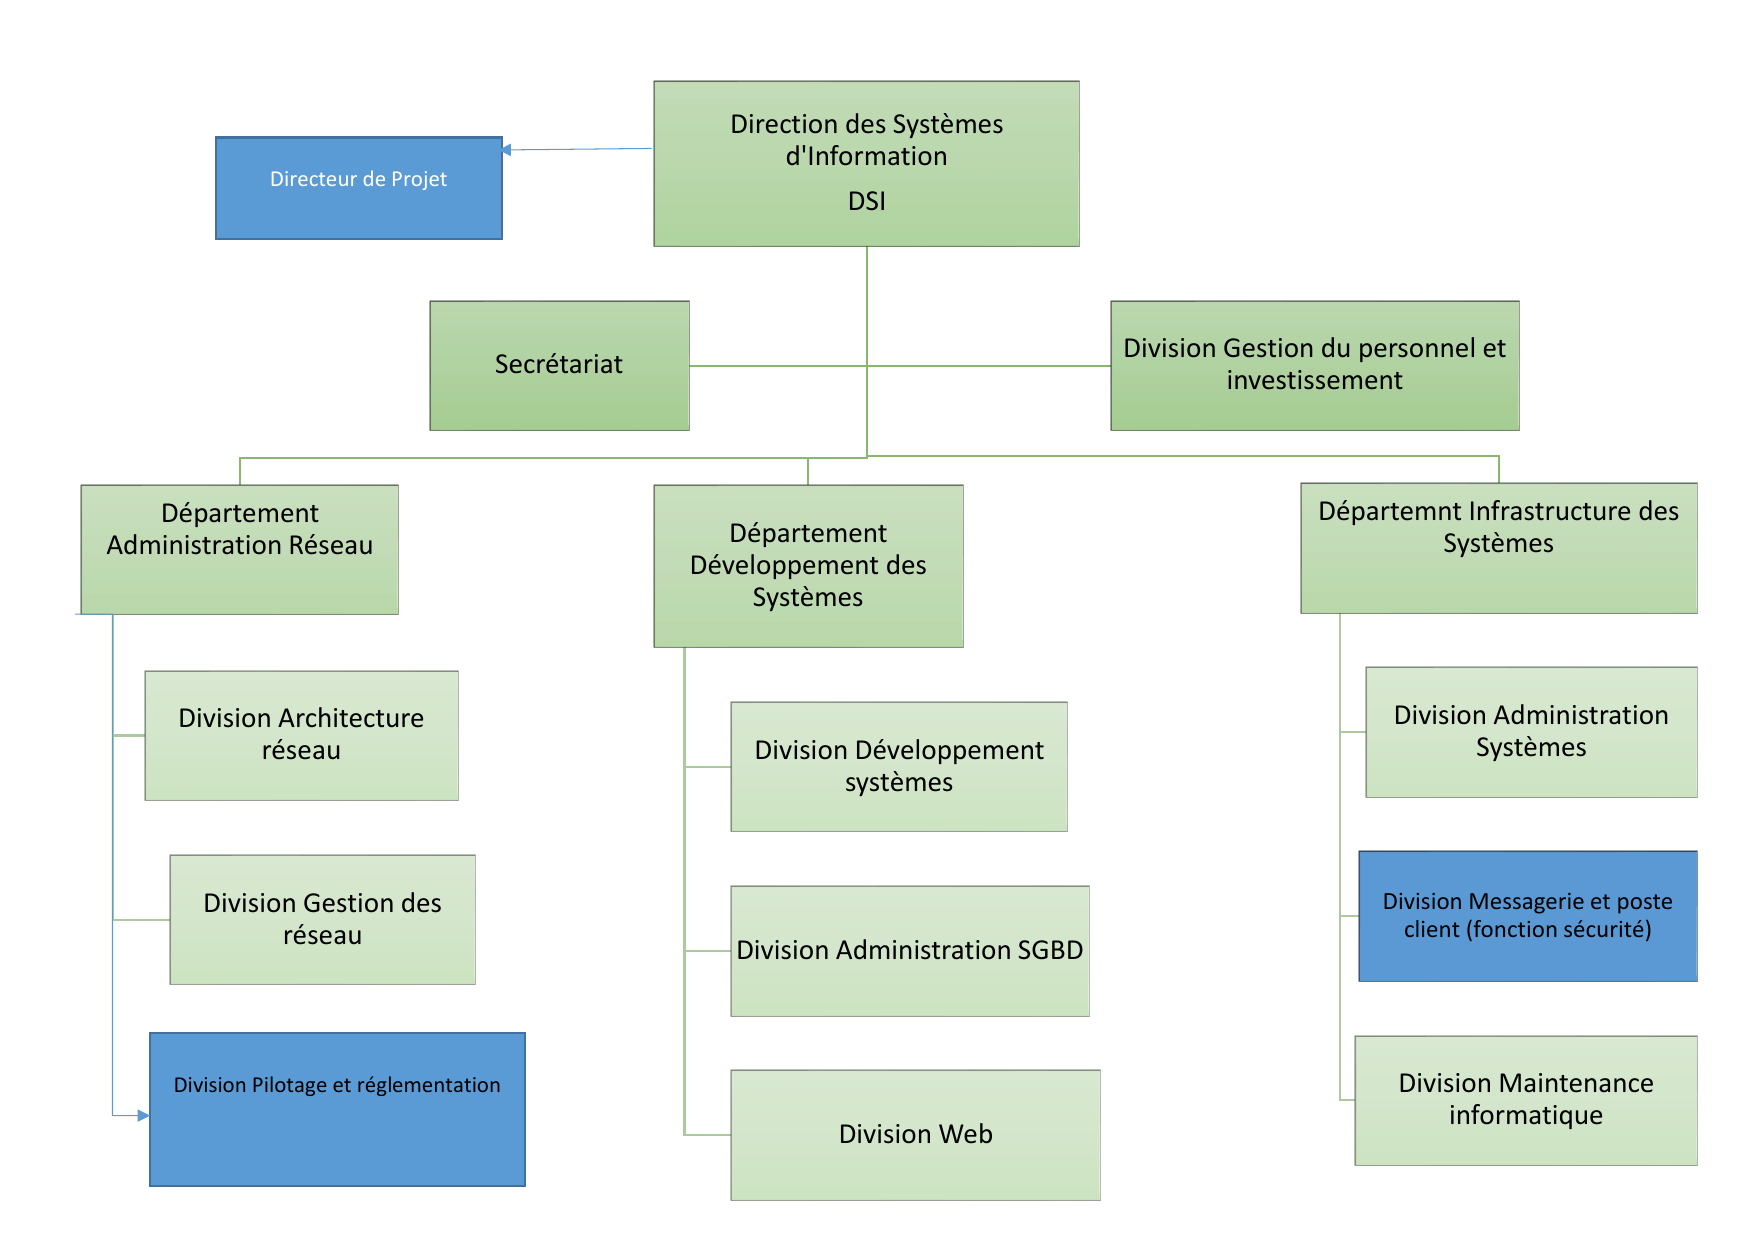
\includegraphics[height=0.86\textheight,keepaspectratio]{figures/dsi-organigramme.png}
	\caption{Organigramme of the SNTF DSI}
	\label{fig:sntf-dsi-organigramme}
\end{figure}
\end{landscape}

\subsection{Why SNTF is relevant to MapIT}
Given the nature of their business, a platform like MapIT would serve a natural purpose at SNTF. Railways depend on proper documentation, uninterrupted service, traceability, and coordination among the technical support teams. Operating a geographically dispersed transport network creates additional need to organize the knowledge systematically, and create visibility regarding assets, incidents, and inter-component relationships. Consequently, MapIT fits into the documentation requirements of a large enterprise.
\section{General Context}
In the world of today, IT infrastructures are deployed on servers, virtual machines, services, network devices, knowledge articles, and incident entries. In the codebase of MapIT, this diversity is evident in that there are specific routes for \texttt{/assets}, \texttt{/incidents}, \texttt{/problems}, \texttt{/relationships}, \texttt{/search}, \texttt{/reports}, and \texttt{/settings}, while the backend provides corresponding API modules for each domain. An IT platform in this environment requires more than merely displaying the data: it is meant to structure the technical memory for support specialists who are able to grasp dependencies, respond fast, and maintain the rationale behind their operations.
\section{Problem Statement}
\subsection{The operational gap}
The main problem solved by MapIT is the absence of a comprehensive, visualized environment for documenting knowledge about IT assets and incidents. In many real-life teams, asset data resides in one system, incident records live in another, and solutions are stored in yet a third source. The lack of integration makes it impossible for a support engineer to have the whole picture at hand: which asset was affected, which components depend on it, in which incident the same problem occurred before, and which document could be reused for the solution.

\subsection{Why the gap matters}
When the technical knowledge is fragmented into multiple documents, the same diagnostics has to be performed several times, the response is delayed, and organizational memories get lost. On top of that, it gets difficult to perform audits, assign responsibility, and track the progress of problem solving in time. In MapIT, these issues are handled through linking incidents with assets, problems, documents, and relationships, as well as through auditing permission related events.
\subsection{What is specific to MapIT}
MapIT is a specialized platform, not a generic content management system. It solves an issue with documentation in IT operations: lack of a single repository where knowledge would be available both in text and in graphs. The idea of linking an incident, problems, solutions, assets, and relations between them is precisely what makes MapIT unique. Thus, the operational gap that this project aims to fill is that of IT infrastructure knowledge management.
\section{Motivations and Project Relevance}
\subsection{Academic motivation}
From an academic point of view, the project is interesting since it combines major aspects of a specialization in Computer Systems: information systems analysis, relational data modeling, API design, authentication, access permissions, and front-end interface development. Following this logic, it can be seen that MapIT represents a good choice as a topic for an academic project.
\subsection{Professional motivation}
On a professional level, MapIT reflects the type of platform that technical support teams use for maintaining IT infrastructure. The platform includes a dashboard with summaries, asset inventory, incident life cycle management, knowledge/problem pages, graph visualization of relations, report generation, and access-controlled settings. This behavior is typical of knowledge platforms but not of brochure-like websites. Therefore, the project is relevant for a real-world IT environment and can be seen as a prototype for a practical solution to a common problem in the industry.
\section{Our Role as Computer Science Students Specializing in Computer Systems}
\subsection{Academic role}
As Computer Science students specializing in Computer Systems, our role was to turn a real operational need into a formal software architecture and then into a working implementation. This involved understanding the domain, defining the data model, specifying the access rules, and implementing the frontend and backend in a way that remains coherent and maintainable.

\subsection{Technical role}
The code shows that our technical role was broader than writing pages: we had to design the Prisma schema, implement JWT-based authentication with LDAP support in production and dev credentials in development, enforce permissions through middleware, and make the frontend consume the API through a Next.js proxy route. These tasks reflect a systems-oriented skill set because they connect infrastructure understanding with application engineering.

\section{Project Objectives and Scope}
\subsection{Functional objectives}
The immediate objectives of MapIT are to authenticate users, show an operational dashboard, manage assets, track incidents, document reusable problems and solutions, display infrastructure relationships, search across all knowledge types, and provide reporting and settings screens. The codebase confirms that each of these capabilities has a dedicated route and user interface.

\subsection{Scope of the first phase}
The current phase focuses on the essential operational workflow. It already includes login, dashboard summaries, incident list and detail views, asset inventory, knowledge/problem pages, relationship visualization, global search, reports, and settings. More advanced features such as richer analytics, automated workflows, or deeper notification logic can be introduced later without changing the core model.

\subsection{Planning and work organization}
The work was organized in successive phases: requirements analysis, study of existing solutions, theoretical framing, conception, modeling, implementation, and validation. This phased organization ensured that each deliverable was produced in the right order and that technical decisions remained aligned with the project objectives.

\section{Chapter Conclusion}
This chapter established that MapIT solves a concrete infrastructure knowledge problem: the absence of a centralized, visual, and role-aware place to manage assets, incidents, and reusable technical knowledge. The next chapter reviews the theoretical concepts that justify this architecture, especially information systems, knowledge management, incident tracking, and relationship mapping.
